%!TEX TS-program = xelatex
%!TEX encoding = UTF-8 Unicode

%%
%% 使用 njuthesis 文档类生成南京大学本科生毕业论文的示例文档
%% 
%%

%% 
%% 南京大学本科学位论文模板
%% 2018年封面,摘要都发生了变化,本模板由以下2016年模板更改而来:http://haixing-hu.github.io/nju-thesis/

%% 如需Adobe字体请用(默认)
%\documentclass[adobefonts]{njuthesis}
%% MacOS系统请用
%\documentclass[macfonts]{njuthesis}
%% Windows系统请用
\documentclass[winfonts]{njuthesis}
%% Linux系统请用
%\documentclass[linuxfonts]{njuthesis}

%%%%%%%%%%%%%%%%%%%%%%%%%%%%%%%%%%%%%%%%%%%%%%%%%%%%%%%%%%%%%%%%%%%%%%%%%%%%%%%
% 设置论文的中文封面
% 论文标题
\title{分析和仿真带权拥塞控制算法}

% 论文作者姓名
\author{吴昌容}
% 论文作者学号
\studentid{161220134}
% 导师姓名职称
\supervisor{田臣}
% 导师职称
\supervisortitle{副教授}
% 论文作者院系
\department{计算机科学与技术系}
% 论文作者专业方向
\major{计算机科学与技术}
% 论文作者的年级
\grade{2016级}
% 论文提交日期,需设置年、月、日。此属性可选,默认值为最后一次编译时的日期,精确到日。
\submitdate{2020年5月22日}

%%%%%%%%%%%%%%%%%%%%%%%%%%%%%%%%%%%%%%%%%%%%%%%%%%%%%%%%%%%%%%%%%%%%%%%%%%%%%%%
% 设置论文的英文封面

% 论文的英文标题
\englishtitle{Simulation and Analysis of Weighted Congestion Control Algorithms}
% 论文作者姓名的拼音
\englishauthor{Changrong Wu}
% 导师姓名职称的英文
\englishsupervisor{Associate Professor Chen Tian}
% 论文作者所在院系的英文名称
\englishdepartment{Department of Computer Science and Technology}
% 论文作者所在学校或机构的英文名称。此属性可选,默认值为``Nanjing University''。
\englishinstitute{Nanjing University}
% 论文完成日期的英文形式,默认最后一次编译的时间
\englishdate{May 22, 2020}
% 专业
\englishinstitute{Computer Science and Technology}
%%%%%%%%%%%%%%%%%%%%%%%%%%%%%%%%%%%%%%%%%%%%%%%%%%%%%%%%%%%%%%%%%%%%%%%%%%%%%%%
% 设置论文的页眉页脚
\usepackage{fancyhdr}
\pagestyle{fancy}
\lhead{\bfseries 161220134 }
\chead{分析和仿真带权拥塞控制算法}
\rhead{吴昌容}
\renewcommand{\headrulewidth}{0.4pt}
%\renewcommand{\footrulewidth}{0.4pt}
%%%%%%%%%%%%%%%%%%%%%%%%%%%%%%%%%%%%%%%%%%%%%%%%%%%%%%%%%%%%%%%%%%%%%%%%%%%%%%%
\begin{document}

% 制作中文封面
\maketitle
% 制作英文封面
% \makeenglishtitle
% 毕业论文过程管理四页表
%\controlpage %可以将word文件交给老师签字后扫描转成pdf,然后命名为controlpage.pdf

% 论文的中文摘要
\begin{abstract}
  拥塞控制是传输层协议TCP(Transmission Control Protocol)的核心组成部分。一般的拥塞控制算法追求公平性,即希望能在每一条参与竞争的网络流中平均分配带宽。而带权拥塞控制(又称加权拥塞控制)算法则是普通拥塞控制算法的拓展,其试图用端到端的方式来在TCP流中按流的权重来分配带宽。计算机网络界的前辈们已经提出了两种著名的带权拥塞控制算法——MulTCP和EWTCP。由于基于加增乘减的拥塞控制算法的公平性最易于掌控,所以这两种算法均是希望通过调整TCP流的加增乘减机制来实现加权公平性。然而在科研实验中,我发现这些经典的加权拥塞控制算法并不总是能很好地按权重来分配带宽。事实上,在不同的环境条件下它们的表现会出现极大的区别。在本论文中,我将会呈现MulTCP和EWTCP两种加权拥塞控制算法的仿真实验结果,并分析其行为和性能变化。我会用实验数据说明加权拥塞控制算法的性能实际上会受到交换机缓冲区大小和链路传播时延的严重影响。最后,我总结出了这两种加权拥塞控制算法的表现随环境因素变化的规律。
% 同时应该注意到,空白页是故意留白,以便章节开头能够出现在偶数页。
% 中文关键词。关键词之间用中文全角分号隔开,末尾无标点符号。
\keywords{拥塞控制;带宽分配;加权公平性}
\end{abstract}

%%%%%%%%%%%%%%%%%%%%%%%%%%%%%%%%%%%%%%%%%%%%%%%%%%%%%%%%%%%%%%%%%%%%%%%%%%%%%%%
% 论文的英文摘要
\begin{englishabstract}
  Congestion Control is one of the critical components of TCP (Transmission Control Protocol). Normal congestion control algorithms aim to achieve fairness among all competing flows, which means they will try to allocate a fair share of the link capacity to each flow. Weighted congestion control algorithms are extensions of the normal versions. Basically speaking, weighted congestion control algorithms aim at using end-to-end mechanisms to allocate bandwidth proportionally according to flows’ weights. MulTCP and EWTCP are two representative schemes of weighted congestion control algorithms. Since the fairness of AIMD-based congestion control algorithms is most comprehensible, both of the schemes attempt to achieve weighted proportionality via modifying the behavior of AIMD (Additive Increase Multiplicative Decrease). However, in real experiments, I find that those weighted congestion control algorithms have variable performance in different circumstances. In fact, their performance with regard to weighted proportionality fluctuates drastically in various network environments. In this paper, I present the simulation results of MulTCP as well as EWTCP and analyze the variation of their behaviors and performance. I will show that both switch buffer size and propagation delay can significantly affect the performance of AIMD-based weighted congestion control algorithms, while these environmental parameters do not influence flows’ behaviors. Finally, I will conclude the pattern of weighted congestion control algorithms’ performance variation. 
% 英文关键词。关键词之间用英文半角逗号隔开,末尾无符号。
\englishkeywords{Congestion Control, Bandwidth Allocation, Weighted Fairness}
\end{englishabstract}

%%%%%%%%%%%%%%%%%%%%%%%%%%%%%%%%%%%%%%%%%%%%%%%%%%%%%%%%%%%%%%%%%%%%%%%%%%%%%%%
% 论文的前言,应放在目录之前,中英文摘要之后
%
\begin{preface}

这是对我本科科研成果的一个提炼和总结。

\vspace{1cm}
\begin{flushright}
吴昌容
2020年5月22日于广西南宁
\end{flushright}

\end{preface}

%%%%%%%%%%%%%%%%%%%%%%%%%%%%%%%%%%%%%%%%%%%%%%%%%%%%%%%%%%%%%%%%%%%%%%%%%%%%%%%
% 生成论文目录
\tableofcontents

%%%%%%%%%%%%%%%%%%%%%%%%%%%%%%%%%%%%%%%%%%%%%%%%%%%%%%%%%%%%%%%%%%%%%%%%%%%%%%%
% 生成插图清单。如无需插图清单则可注释掉下述语句。
%\listoffigures

%%%%%%%%%%%%%%%%%%%%%%%%%%%%%%%%%%%%%%%%%%%%%%%%%%%%%%%%%%%%%%%%%%%%%%%%%%%%%%%
% 生成附表清单。如无需附表清单则可注释掉下述语句。
%\listoftables

%%%%%%%%%%%%%%%%%%%%%%%%%%%%%%%%%%%%%%%%%%%%%%%%%%%%%%%%%%%%%%%%%%%%%%%%%%%%%%%
% 开始正文部分
\mainmatter

%%%%%%%%%%%%%%%%%%%%%%%%%%%%%%%%%%%%%%%%%%%%%%%%%%%%%%%%%%%%%%%%%%%%%%%%%%%%%%%
% 学位论文的正文应以《绪论》作为第一章
\chapter{绪论}\label{chapter:introduction}
\section{研究背景}
拥塞控制(Congestion Control)是传输层协议TCP(Transmission Control Protocol)的核心组成部分。
在TCP的整体控制系统中,拥塞控制担负着解决网络拥塞和避免丢包以提升网络性能的重要责任\cite{jacobson1988congestion}。
公平性是拥塞控制算法的主要性质之一,其要求拥塞控制算法能够在互相竞争的网络流中公平地分配带宽。
由于公平性不仅是个技术问题还是个社会问题,公平性从传输层控制协议(TCP)加入拥塞控制算法伊始,就一直为人们所关注。
在拥塞控制算法和理论发展的早期,人们主要关注如何才能使TCP拥塞控制算法达到公平性以及某种拥塞控制算法是否满足公平性的要求等问题\cite{chiu1989analysis}\cite{kelly1998rate}\cite{hasegawa1999fairness}。
但是随着网络的发展,在某些新的应用场景\cite{wischik2011design}\cite{Nathan2019wcubic}下,人们其实并不是希望公平地分配带宽而是希望能按权重来分配带宽。
因此,研究者们又进一步关注到了公平性的广义拓展——加权公平性。
具有加权公平性的拥塞控制算法就是带权拥塞控制或加权拥塞控制(Weighted Congestion Control)算法,这种算法根据每条网络流的权重来分配带宽。
由于基于加增乘减机制的拥塞控制算法的公平性最易于掌控和理解,最经典的两种带权拥塞控制算法MulTCP\cite{crowcroft1998differentiated}和EWTCP\cite{wischik2011design}也都是基于加增乘减机制的。
加增乘减(Additive Increase Multiplicative Decrease)机制是TCP协议拥塞控制的主要方法,它结合了线性探索和乘性退避的功能。
而且,加增乘减机制已经被证明可以保证每条参与竞争的TCP流都一定会收敛到公平的均衡点~\cite{chiu1989analysis}。
本文也将主要关注MulTCP和EWTCP这两种经典的基于加增乘减机制的带权拥塞控制算法。

\section{研究动机}

如今网络服务已经由free-use模型发展到pay-for-use模型,传统的公平性应当增强为加权公平性,以实现基于不同价格的差异化服务。
首先,为了支持日渐增多的异质化应用对网络带宽的不同要求,网络管理者往往需要在网络中为不同的流量配置优先级或权重\cite{Hong2013SWAN}。
拥有较高权重的流在竞争有限的带宽资源时,应该获得比权重较低的流更多的带宽。
其次,在数据中心中网络带宽应该按照每个租户支付的金钱来进行分配\cite{popa2012faircloud}。
如果一个租户支付了更高的服务费用,那么它理应获得更多的带宽。
加权拥塞控制正是一种可以用端到端的方式、简单高效地实现差异化服务的机制。
而且加权拥塞控制还可以从最细粒度的流一级上去控制带宽,并具有工作保留(Work-Conserving)的特性。
比如,如果能用加权拥塞控制来实现\cite{popa2012faircloud}中的带宽分配系统,那么将极大地提升系统的可拓展性,并降低交换机队列资源的消耗。
\cite{Nathan2019wcubic}中也正是使用加权拥塞控制来实现了更高粒度的用户体验质量(Quality of Experience)层级的公平性。
因此,我们希望能分析出加权拥塞控制的一些特性和规律,以便为带宽分配系统的设计提供指导。

\section{相关工作}

现有的支持网络带宽差异化分配的工作主要是利用交换机上的队列资源来对流量进行调度从而实现按权或按优先级分配带宽,比如Weighted Fair Queuing(WFQ)\cite{demers1989analysis}\cite{Abhay1993WFQ}和Diffserv\cite{Kathleen1998Diffserv}。
前几年提出的NUMFabric\cite{nagaraj2016numfabric}和Faircloud\cite{popa2012faircloud}均依赖于交换机上的WFQ来实现加权公平性。
功能日渐强大的交换机确实可以帮助实现加权公平性,但对交换机的依赖也使得这些系统的部署受到了限制。
由于网络节点总是要对网络的反馈作出回应,因此以加权拥塞控制为代表的端到端速率调整机制其实对于实现加权公平性更为普适和重要。
MulTCP\cite{crowcroft1998differentiated}和EWTCP\cite{wischik2011design}就是两种典型的基于AIMD的加权拥塞控制算法。
它们均通过在端上修改TCP拥塞控制的加增乘减机制来实现差异化带宽分配。
MulTCP根据锯齿模型分析得出的结论\cite{Floyd1997Sawtooth}提出:对于权重为$w$的TCP流,其加增参数和乘减参数应当分别为$w$和$1-\frac{1}{2w}$。
事实上MulTCP是存在问题的,因为其理论模型是基于每一条流拥塞窗口的变化均是高度同步这一假设的,而这个假设是不符合实际的。
EWTCP的设计想法则是来自于TCP流带宽随机测量模型\cite{padhye1998modeling},对于权重为$w$的TCP流,它在普通加增乘减的基础上将加增的参数改为$w$。
EWTCP使用的模型在特定的情形下确实能够对单条TCP流的带宽进行较为准确地测量,但是这种模型没有将网络中动态变化的排队时延考虑进去。
因此,当交换机中队列的长度发生改变时,这种模型就会与现实产生偏差。
总的来说,MulTCP和EWTCP都只是提出了一种基于AIMD的加权拥塞控制算法,而这些算法都没有能够完美地实现加权公平性。
这主要是因为之前的这两份工作\cite{crowcroft1998differentiated}\cite{wischik2011design}都忽视了交换机缓冲区大小、传播时延和ACK选项对流的权重的影响。

\section{本文主要工作}
本文旨在对图片级手写中文文本做出识别分类。主要工作如下:
\begin{enumerate}
\item 在标准公开数据集里获得了一定的识别准确度。

\item 在标准公开数据集上击败了一些相关工作的结果。

\item 建立分本分行规划表格,很好地处理了文本的分行,降低了训练开销。

\end{enumerate}
\section{本文结构}
本文的各章节组织结构如下:

第一章:绪论。简要说明了手写中文文本识别的研究来由及相关工作。并概括地描述了这篇文章的工作,总结了本文结构。

第二章:识别系统

第三章:实验。介绍了实验进行的配置环境,文中使用的测度,文本分行的结果,识别的结果并分析了得到这种结果背后的缘由。

第四章:总结与讨论。总结全文工作,讨论存在的问题和今后可以继续研究的方向。

\chapter{系统}\label{chapter_system}

怎么使用这个模板

\section{图片}

一行一图,如图\ref{fig:line}
\begin{figure}[htbp]
   \centering
   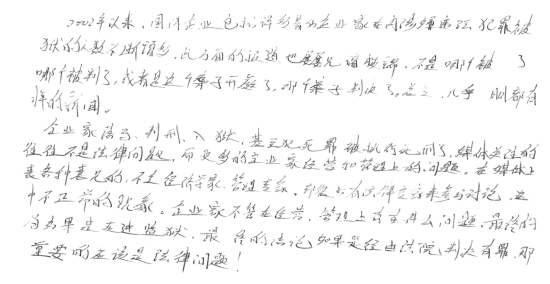
\includegraphics[width=0.7\textwidth]{line.png} % requires the graphicx package
   \caption{待分行文本}
   \label{fig:line}
   %\vspace{0.8cm} % 用来调整和下方文字的间距
\end{figure}


一行两个图
\begin{figure}[ht!]
    \centering
    \begin{subfigure}{.5\textwidth}
    	\centering
        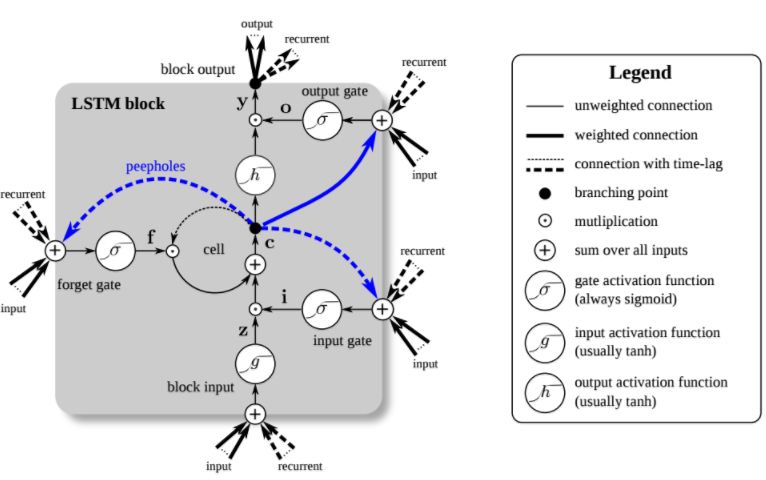
\includegraphics[width=0.9\textwidth]{lstm1.png}
        \caption{长短时记忆单元模块}
    \end{subfigure}
    \begin{subfigure}{.4\textwidth}
    	\centering
        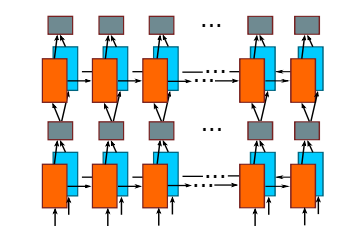
\includegraphics[width=0.8\textwidth]{lstm2.png}
        \caption{深双向长短时记忆}
        \label{fig:lstm2}
    \end{subfigure}
    \caption{(a)一个长短时记忆单元模块。(b)深度双向长短时记忆的结构。}
\label{fig:lstm}
\end{figure}

多行多图
\begin{figure}[ht!]
    \centering
    \begin{subfigure}{\textwidth}
        \centering
        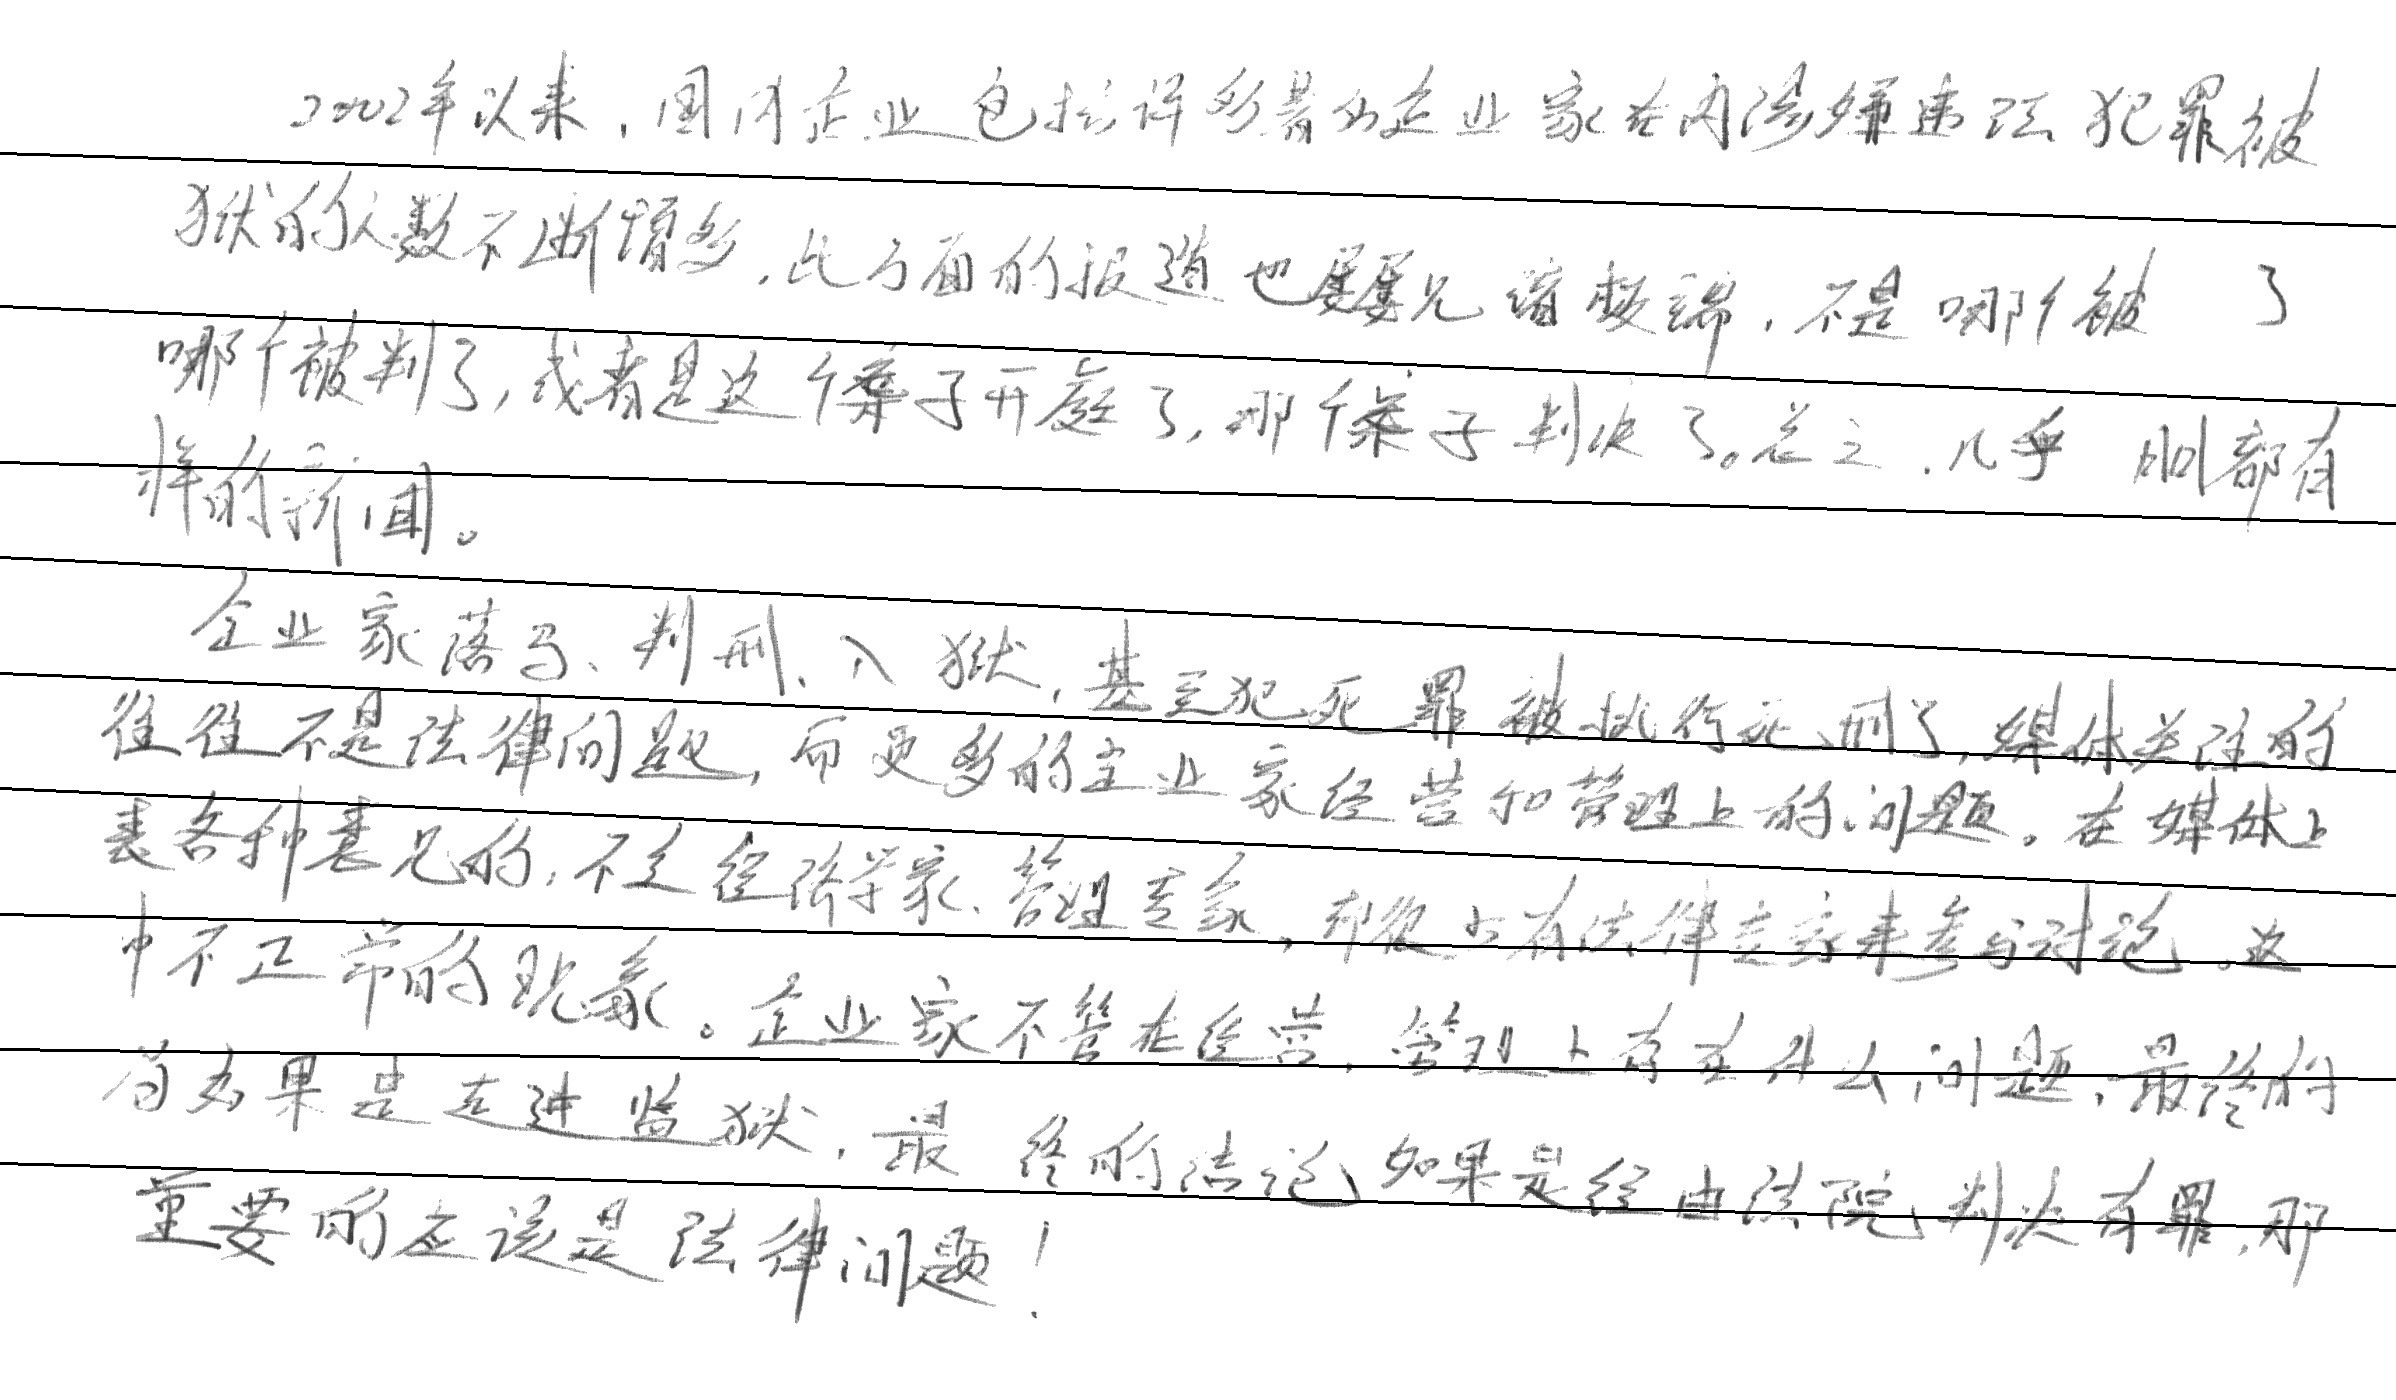
\includegraphics[width=0.59\textwidth]{line1.png}
        \caption{全局损失切割}
        \label{fig:line1}
    \end{subfigure}
    \begin{subfigure}{\textwidth}
    	\centering
        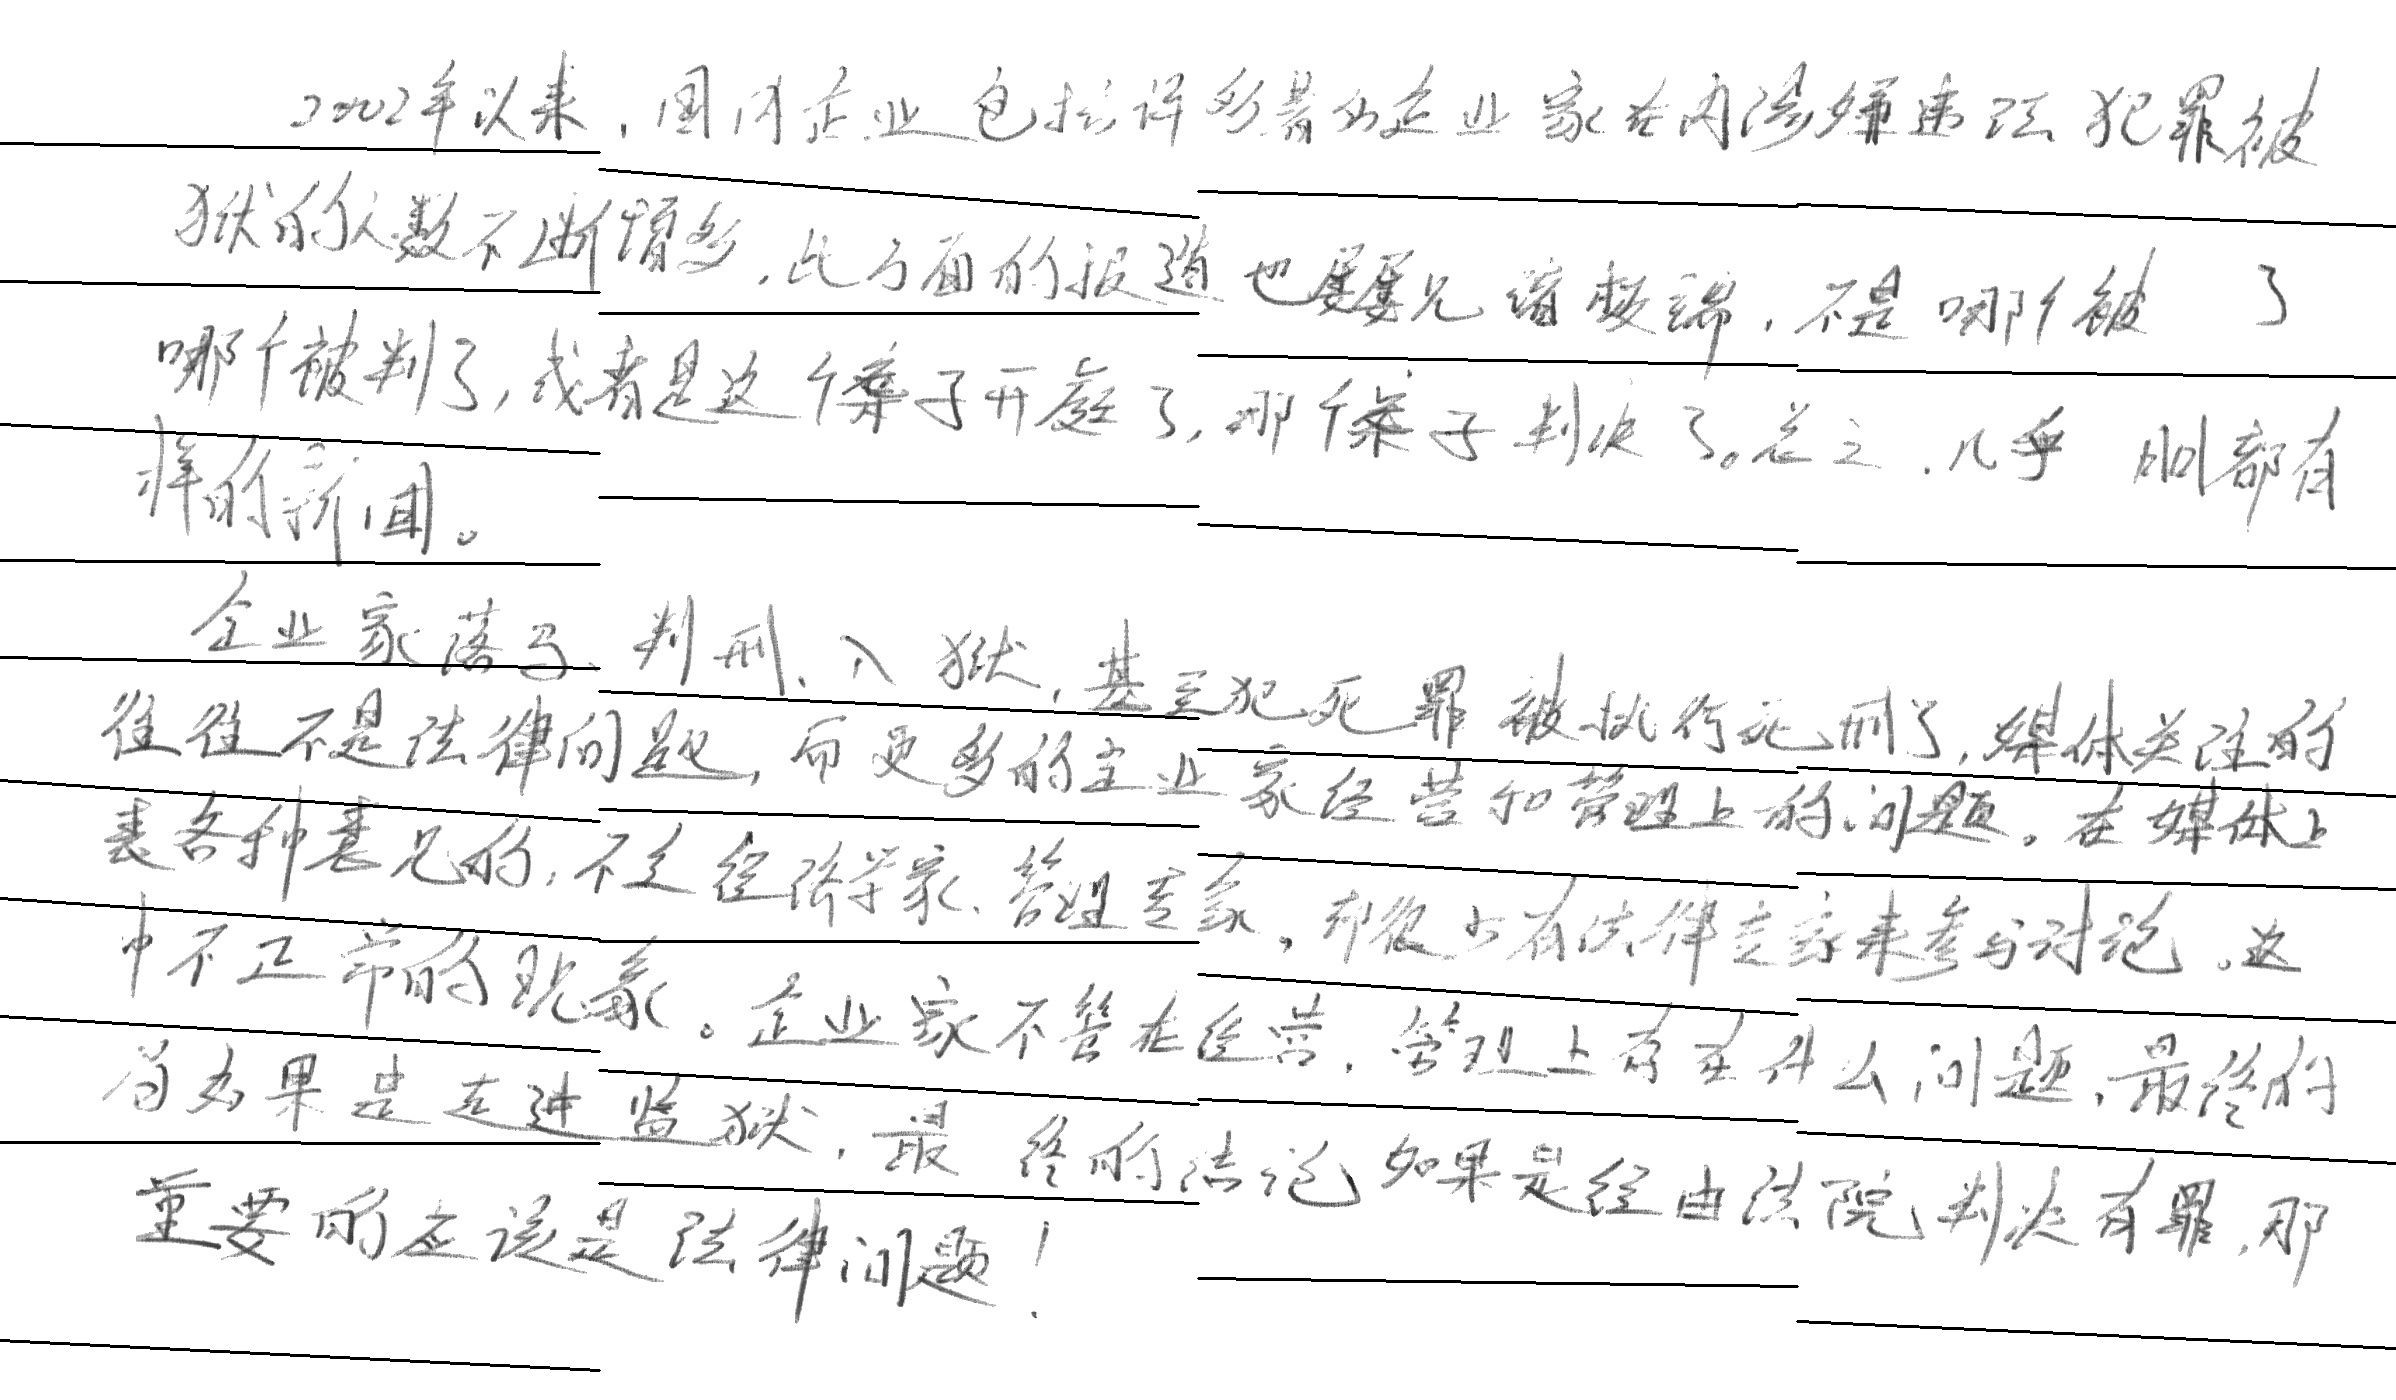
\includegraphics[width=0.59\textwidth]{line2.png}
        \caption{局部损失切割}
        \label{fig:line2}
    \end{subfigure}
    \caption{分行结果比较。(a)全局损失切割;(b)局部损失切割;(c)局部水平投影切割;(d)投影损失切割}
\end{figure}

\newpage %为了将图片实例放在一起,另起一页,使用时请删掉


\section{公式}

\begin{equation}
\frac{\partial L}{\partial a_{k}^t} = {d(s)}^2 (y_{k}^t - \frac{\sum_{lab(\mathbf{l},k)} \alpha_t(s)\beta_t(s) }{y_{k}^t} )
\end{equation}

\begin{equation}
\begin{aligned}
d_{{0j}}&=\sum _{{k=1}}^{{j}}w_{{\mathrm  {ins}}}(a_{{k}}),\quad &{\text{for}}\;1\leq j\leq n\\
d_{{ij}}&={\begin{cases}d_{{i-1,j-1}}&{\text{for}}\;a_{{j}}=b_{{i}}\\\min {\begin{cases}d_{{i-1,j}}+w_{{\mathrm  {del}}}(b_{{i}})\\d_{{i,j-1}}+w_{{\mathrm  {ins}}}(a_{{j}})\\d_{{i-1,j-1}}+w_{{\mathrm  {sub}}}(a_{{j}},b_{{i}})\end{cases}}&{\text{for}}\;a_{{j}}\neq b_{{i}}\end{cases}}\quad &{\text{for}}\;1\leq i\leq m,1\leq j\leq n.
\end{aligned}
\end{equation}

\begin{equation}
\begin{aligned}
&\beta_T(|l{}'|)=y_{b}^{T}\\
&\beta_T(|l{}'|-1)=y_{l_|l|}^{T} \\
&\beta_T(s)=0, \forall s < |l{}'|-1
\end{aligned}
\end{equation}

递归公式
\begin{equation}
\beta_t(s)=\left\{
\begin{aligned}
& (\beta_{t+1}(s) d(s)+\beta_{t+1}(s+1))d(s+1)\,  y_{\l_s{}'}^t, \: \: if \:  l_s{}'=b \:  or \:  l_{s+2}{}'=l_s{}'\\
& (\beta_{t+1}(s) d(s)+\beta_{t+1}(s+1)d(s+1)+\beta_{t+1}(s+2)d(s+2))\,  y_{\l_s{}'}^t,\: \:   otherwise
\end{aligned}
\right.
\end{equation}

\section{表格}

\begin{table}[htbp]
\setlength{\belowcaptionskip}{7pt}
  \centering
\begin{tabular}{|c|c|c|c|c|c|c|c|c|c|}
\hline 
  &   & 国 & 内 & 企 & 业 & 包 & 括 & 许 & 多 \\ 
\hline 
  & 0 & 1 & 2 & 3 & 4 & 5 & 6 & 7 & 8 \\ 
\hline 
国 & 1 & 0 & 1 & 2 & 3 & 4 & 5 & 6 & 7 \\ 
\hline 
著 & 2 & 1 & 1 & 2 & 2 & 3 & 4 & 5 & 6 \\ 
\hline
\end{tabular} 
\vspace{0.2cm}
  \caption{编辑距离(乐文斯汀距离计算过程示例表格。字符串``国内企业包括许多''与``国著名括许多''乐文斯汀距离是3。}\label{table:ld}
\end{table}


\section{算法}

\begin{algorithm}
\caption{Beam Search}
\label{alg:beam}
\begin{algorithmic}[1]
\STATE {将初始节点插入到集束中。} 
\WHILE{遍历未结束}
\STATE {遍历集束中所有节点的后续节点。} 
\IF{该节点是目标节点}
\STATE {算法结束。}
\ELSE 
\STATE {扩展该节点,取集束宽度的节点入堆。}
\ENDIF
\ENDWHILE
\end{algorithmic}
\end{algorithm}

集束宽度可以在搜索过程中保持为一个定值,也可以根据搜索的进行而变化。搜索算法可以根据搜索的结果进行调整,比如,当以一个小的集束宽度搜索解却无法找到适合解的时候,可以增大集束宽度重新进行一次搜索。



\chapter{实验}

\section{实现细节}
我们在Tensorflow框架上实现了我们的网络系统。实验在一个搭载2.40GHz 英特尔志强 Xeon E5-2673 CPU,32GB RAM 和一块英伟达1080Ti 12GB 显存的服务器电脑上运行。网络系统使用Adam训练算法。



\section{文本分行结果}
尽管如此,在局部损失切割和局部水平投影切割之后,每一个竖直段的分行结果的对应关系却很难处理。在一些特殊情况下,无法做到每一竖直段分行关系的对应。所以这两个方法不适用。




\section{识别结果}

\subsection{准确率}
我们根据数据集中人的笔迹将数据集分为了\textbf{HWDB1}-\textbf{HWDB3},并实现了Wang 等人\cite{wang2012end} 和Mishra 等人\cite{mishra2012scene}的方法,通过调用百度的文字识别系统\cite{baiduapi},进行对比实验得到以下结果。

\vspace{0.2cm}
\begin{table}[htbp]
\setlength{\belowcaptionskip}{5pt}
  \centering
  \begin{tabular}{cccc}
    \toprule
    \textbf{方法} & \textbf{HWDB1} & \textbf{HWDB2} & \textbf{HWDB3} \\
    \midrule
    Wang 等人\cite{wang2012end}   			& 74.0 & 60.0 & 68.0  \\
    Mishra 等人\cite{mishra2012scene}		 	& 80.8 & 63.6 & 73.5  \\
    百度通用文字识别\cite{baiduapi}		& 64.8 & 36.8 & 60.8 \\
    \midrule
    我们的方法(没有字典信息)& 81.5 & 67.5 & 73.6  \\
    我们的方法	  		& \textbf{81.8} & \textbf{67.8} & \textbf{73.9}  \\
    \bottomrule
  \end{tabular}
  \vspace{0.2cm}
  \caption{识别准确率}\label{table:result}
\end{table}



\chapter{总结与讨论}
在本文中,我们使用预处理层-卷积层-循环卷积层-转录层网络来处理手写中文文本识别的问题。这种网络很好地结合了卷积网络和循环网络各自的优势。

\bibliography{reference}

%%%%%%%%%%%%%%%%%%%%%%%%%%%%%%%%%%%%%%%%%%%%%%%%%%%%%%%%%%%%%%%%%%%%%%%%%%%%%%%
% 致谢,应放在结论之后
\begin{acknowledgement}
感谢在实验室度过的两年时光,老师无论在学术还是人生的指导上都对我起到了很大的帮助;师兄师姐小伙伴们的鼓励支持和陪伴是我坚持下去的动力。
\end{acknowledgement}

%%%%%%%%%%%%%%%%%%%%%%%%%%%%%%%%%%%%%%%%%%%%%%%%%%%%%%%%%%%%%%%%%%%%%%%%%%%%%%%
\end{document}
